%  !TeX  root  =  user_guide.tex

\section{Оффлайновое редактирование}\label{sec:offlinedit}

% when the revision of a section has been finalized,
% comment out the following line:
%\updatedisclaimer

Во время полевых работ часто приходится использовать ноутбук или коммуникатор
в режиме оффлайн. При возвращении, сделанные изменения необходимо синхронизировать
с основным источником данных, например базой данных PostGIS. Если несколько
человек работает с таком режиме с одним и тем же набором данных, процесс
синхронизации и слияния значительно усложняется, даже если редактировались
разные объекты.

Модуль \toolbtntwo{offline_editing_copy}{Оффлайновое редактирование} автоматизирует
процесс синхронизации, копируя содержимое основного источника данных (обычно,
базы PostGIS или WFS-T) в базу SpatiaLite и сохраняя все правки в специальных
таблицах. При повторном подключении к основному источнику данных, все правки
легко переносятся.

\minisec{Работа с модулем}

\begin{itemize}
\item Загрузите необходимые слои, например из базы PostGIS или сервера WFS-T
\item Сохраните проект
\item Нажмите кнопку <<Преобразовать в оффлайновый проект>> и выберите
слои, которые нужно сохранить. Содержимое слоёв будет записано в базу SpatiaLite.
\item Редактируйте слои.
\item Подключитесь к исходным источника данных снова и загрузите свои правки
нажав <<Синхронизировать>>.
\end{itemize}

\begin{figure}[ht]
   \centering
   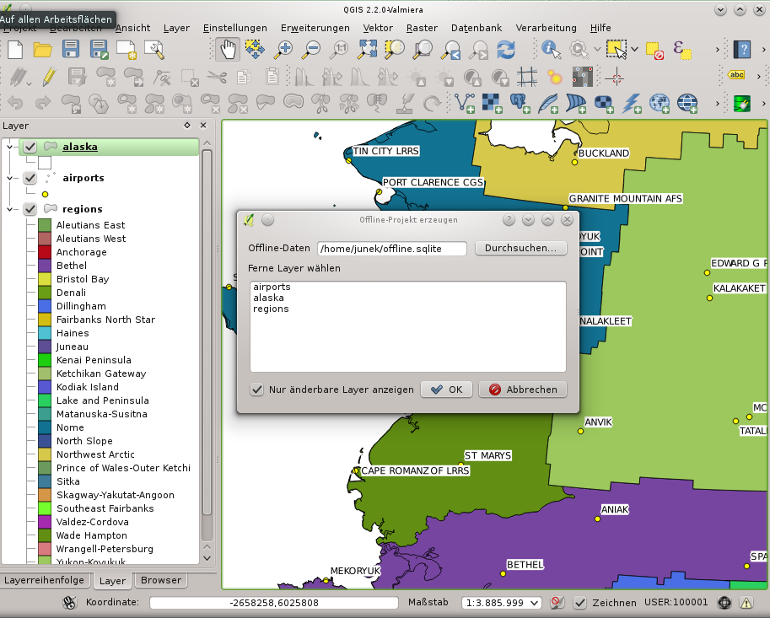
\includegraphics[clip=true, width=12cm]{create_offline_project}
   \caption{Создание оффлайнового проекта из слоёв PostGIS или WFS \nixcaption}
   \label{fig:offlineproject}
\end{figure}

\FloatBarrier
